\chapter{Implementation and Testing}

Jadwal is a fast, and efficient system. It uses technologies that allows it to deliver those promises. The fact that Golang is the main language and that the language is compiled.

\section{Technologies and Tools Used}

Jadwal is built using a carefully selected stack of languages, technologies, and tools that enable fast iteration, strong security, ease of development, and deployment flexibility. Every choice made reflects our priority for speed, maintainability, and a high-quality user experience.

\subsection{Backend}

\begin{itemize}
    \item \textbf{Golang} – The main language used in the backend. It is a compiled language that generates native machine code (not bytecode), providing high performance and low overhead. Go also supports cross-compilation, meaning we can build binaries for different platforms (macOS, Linux, Windows) and architectures (x86, arm64) without requiring physical access to those systems. This was essential for our CI/CD and deployment process.
    \item \textbf{ConnectRPC} – The RPC framework we used to define our API. It is highly efficient and uses Protocol Buffers (protobuf) for serialization. This improves communication speed and ensures a consistent, type-safe interface between backend and frontend.
    \item \textbf{sqlc} – A Go-based SQL compiler. Unlike traditional ORMs that abstract SQL (and often add unnecessary complexity), sqlc lets us write raw SQL while still generating typed Go code. This gives us type safety and full SQL control — the best of both worlds.
    \item \textbf{migrate} – Used to handle schema migrations. Written in Go, it allows us to create up/down migration files and execute them at runtime. We also automated it to run at app startup, making database updates smoother during deployment.
    \item \textbf{RabbitMQ} – Our message broker used to decouple the WhatsApp message extraction service from the backend logic. It provides robust, asynchronous communication with delivery guarantees, retries, and scaling potential.
    \item \textbf{OpenAI-based LLM API} – Used in our event extraction pipeline to analyze and classify incoming WhatsApp messages. The abstraction allows easy model switching in the future without changing core logic.
    \item \textbf{HTTPJ} – A REST utility server that handles lightweight jobs like `.mobileconfig` file downloads. While not a central component, it simplifies small tasks that don’t need full RPC wiring.
    \item \textbf{Baikal} – An open-source CalDAV server written in PHP. It handles calendar data storage and sync and was reused in our system to provide a standards-based calendar integration layer.
\end{itemize}

\subsection{Frontend (iOS)}

\begin{itemize}
    \item \textbf{SwiftUI} – The framework used to build the iOS UI. It offers declarative, responsive UI development and is well-suited for small teams due to its simplicity.
    \item \textbf{EventKit} – Apple's official framework for accessing and managing calendar data on-device. It is used to read events, create prayer reminders, and add WhatsApp-parsed events.
    \item \textbf{Xcode} – Apple's IDE used to build, test, and debug the app. Also used for handling provisioning profiles and release builds.
    \item \textbf{JWT (JSON Web Token)} – Used for stateless authentication. Each user receives a signed token after login, which includes their identity (email/user\_id) and is verified using digital signatures to prevent tampering.
    \item \textbf{APNs (Apple Push Notification Service)} – Used to send push notifications for new events, conflicts, and reminders. We collect device IDs and securely store them to trigger these updates.
\end{itemize}

\subsection{WhatsApp Service (Wasapp)}

\begin{itemize}
    \item \textbf{TypeScript} – The main language for the Wasapp service.
    \item \textbf{bun.sh} – Used as our runtime for TypeScript — fast, modern, and integrates well with our stack.
    \item \textbf{Fastify} – A high-performance Node.js framework used to expose an API to the backend from the Wasapp service.
    \item \textbf{whatsapp-web.js} – JS client library that connects to WhatsApp Web, receives messages in real time, and emits events. This is the heart of our message extraction logic.
\end{itemize}

\subsection{Infrastructure, Deployment, and DevOps}

\begin{itemize}
    \item \textbf{Docker} – Everything runs in containers: backend, Wasapp, CalDAV, etc. This enables consistent environments between dev and production.
    \item \textbf{Docker Compose} – Used to orchestrate services locally and during staging. Ensures that every developer gets the same setup out of the box. We used overlays, to override values between production and local environment along with `.env' files.
    \item \textbf{Traefik} – Our reverse proxy/load balancer/API gateway. It integrates with Docker, automatically issues SSL certs via Let's Encrypt, and handles SSL termination (internal services communicate over HTTP for performance).
    \item \textbf{GitHub} – Our version control system, CI/CD pipeline, and GitOps source of truth.
    \begin{itemize}
        \item \textbf{GitHub Actions} – CI workflows for building, testing, and pushing Docker images to GitHub Packages.
        \item \textbf{GitHub Packages} – Our Docker registry. Stores built images and lets us pull them easily on the server.
        \item \textbf{BlackSmith} – A third-party CI runner provider that gives us faster runners at lower cost. Speeds up builds and saves credits.
    \end{itemize}
    \item \textbf{Cloudflare} – Handles DNS, provides DDoS protection, serves as our CDN edge, and allows cheap domain registration. We also use it to force HTTPS and cache public assets.
    \item \textbf{Taskfile} – A Go-based task runner. We use it to alias common dev commands, test scripts, and deploy workflows into short commands.
\end{itemize}

\subsection{Database and Security}

\begin{itemize}
    \item \textbf{PostgreSQL} – Our main database. Used to store customers, calendar connections, event metadata, WhatsApp messages, device IDs, and more.
    \item \textbf{Beekeeper Studio} – A SQL GUI that lets us explore, debug, and visualize our PostgreSQL database. Used frequently during development.
    \item \textbf{Encryption at Rest (WhatsApp)} – We encrypt WhatsApp messages before storing them to protect user privacy in the case of a breach or access by other services.
    \item \textbf{Scratch Docker Images} – Our Go binaries are compiled statically and run inside Docker images built `FROM scratch`, meaning the containers are literally empty — no shell, no package manager, nothing for an attacker to exploit.
\end{itemize}

\subsection{Design, Documentation, and Diagrams}

\begin{itemize}
    \item \textbf{LaTeX} – Used to write this entire report. It handles figure references, bibliography, equation rendering, and allows us to store the report in version control for collaboration.
    \item \textbf{PlantUML} – Used to make sequence and class diagrams using plain text that can be rendered as SVG or PNG.
    \item \textbf{Mermaid} – Used for Gantt charts and simple flow diagrams, especially in markdown files and web-based previews.
    \item \textbf{Draw.io} – Used when text-based tools are too limited. We still track the `.drawio` files in GitHub for versioning.
    \item \textbf{UMLet} – Lightweight UML diagram tool used to make clean use case diagrams.
\end{itemize}

\subsection{Design and Productivity Tools}

\begin{itemize}
    \item \textbf{Figma} – Used to design our app logo, UI mockups, and presentation slides.
    \item \textbf{VS Code} – Our primary code editor. Supports extensions, Git integration, LaTeX building, and everything else we needed.
    \item \textbf{Linear} – Used for high-level project planning. Initially we tried micro-planning with it, but the project moved too quickly. We stuck to major task tracking and daily syncs.
    \item \textbf{Resend} – A transactional email service. We use it to send welcome emails, magic links, and other system emails. It has a generous free tier and works reliably.
    \item \textbf{PostHog} – A powerful analytics tool that tracks usage funnels, sessions, and user behavior. It enabled us to see session replays and understand user flows without asking users directly.
\end{itemize}

\section{System Architecture (Implemented)}

The system architecture, as originally outlined in Figure \ref{fig:architecture}, was implemented using a modular, containerized structure. All core components were packaged as separate services and deployed using Docker Compose on a single host. These include the backend service (Falak), the WhatsApp service (Wasapp), the CalDAV server (Baikal), a PostgreSQL database, and a Traefik proxy for HTTPS termination and service routing.

While the design envisioned a distributed system, the final implementation runs on a single host with isolated containers communicating over internal Docker networks. This setup preserves modularity and mirrors real-world deployment environments, while simplifying development and debugging. Each service is decoupled and can be scaled independently in future production-grade deployments.

The implemented architecture maintained full alignment with the original design, with minor practical adjustments such as unified logging using Grafana + Loki, simplified internal networking, and local queues (RabbitMQ) for event-driven flows. Overall, the implementation delivered on the designed goals of modularity, maintainability, and separation of concerns.


\section{Database Implementation}

The original database design, illustrated in Figure~\ref{fig:er-diagram} and Figure~\ref{fig:relational-schema}, was adapted during the actual system implementation. Initially, we planned to manage calendar storage directly within our own database schema. However, during development, we decided to integrate Baikal — an open-source, self-hosted CalDAV server — to handle calendar data following the CalDAV standard.

As a result, several tables from the original ERD were removed or replaced. The Falak backend continues to manage user accounts, authentication methods, WhatsApp message extraction, device IDs, and notification tracking, while Baikal independently handles all calendar-related storage.

The updated database design for the Falak backend, reflecting these changes, is shown in Figure~\ref{fig:updated-er-diagram} and Figure~\ref{fig:updated-relational-schema} below.

\begin{figure}[!h]
    \centering
    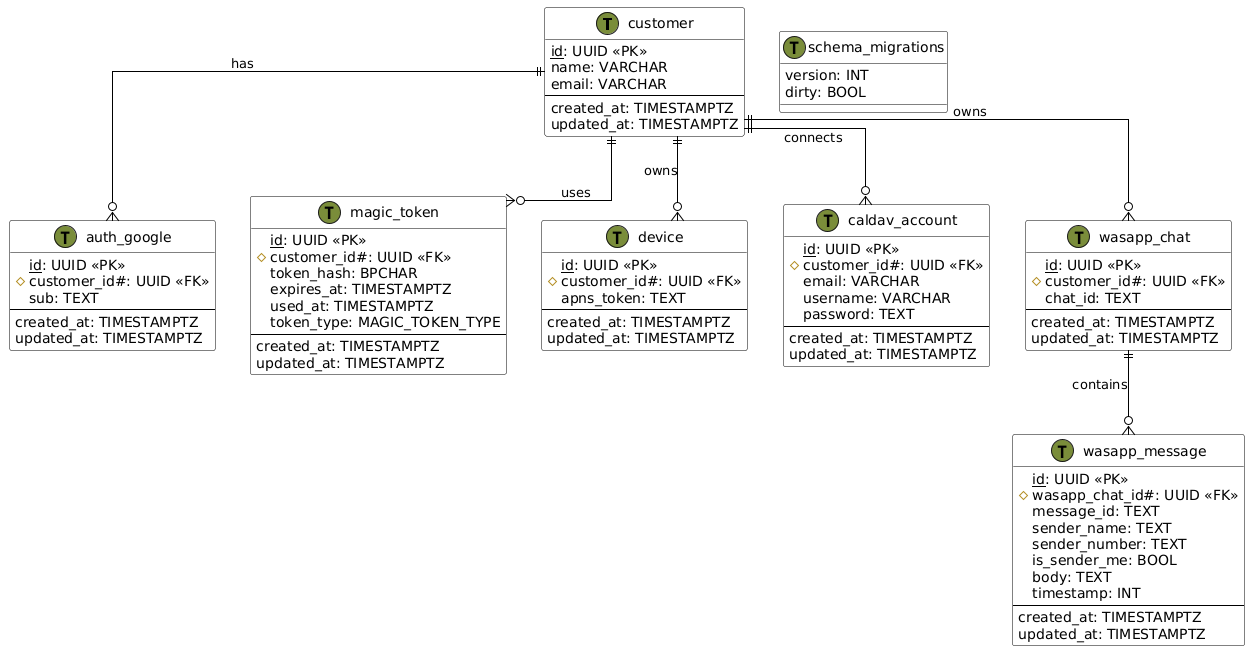
\includegraphics[width=0.9\textwidth]{images/docs/diagrams/er/new-database/Updated Falak ERD.png}
    \caption{Updated Entity-Relationship Diagram (Falak)}
    \label{fig:updated-er-diagram}
\end{figure}

% TODO: make this a relational one with draw.io, based on the one above :D
% \begin{figure}[!h]
%     \centering
%     \includegraphics[width=\textwidth]{images/updated-database-schema-relational.png}
%     \caption{Updated Relational Schema (Falak)}
%     \label{fig:updated-relational-schema}
% \end{figure}

\subsection{Baikal Database Schema}

To handle calendar event storage, we integrated Baikal directly without modifying its schema. Baikal follows WebDAV and CalDAV standards and manages calendars, events, user principals, and contact address books internally.

The key Baikal tables relevant to Jadwal's functionality are summarized below:

\begin{itemize}
    \item \textbf{calendars} — Stores metadata for user calendars.
    \item \textbf{calendarobjects} — Stores individual calendar events in iCalendar format.
    \item \textbf{calendarinstances} — Links calendars to user principals.
    \item \textbf{principals} — Represents authenticated users within Baikal.
\end{itemize}

Other tables related to address books, scheduling, and WebDAV-specific functionality (e.g., locks, subscriptions) were unused in our implementation. Baikal's database provided a mature and reliable backend for event storage without requiring us to reinvent a full calendar system.


\section{Implementation of Core Functionalities}

\subsection{Authentication}
\label{subsec:authentication}
The authentication flow supports both magic links (email-based) and Google OAuth. Users receive a signed JWT upon authentication, which is used for subsequent requests. We call it authenatication since we don't differentiate between making an account and making one. The user just `continues' with a method, either Email with Magic Link or Google OAuth, and if they already have an account we just give them a token, but if they don't have account, we create one for them, send a welcome email, and then give the tokens. 

Regarding the tokens, we generate access tokens (short-lived) and refresh tokens (long-lived), stored securely on the device. Magic tokens are hashed using SHA-256 before being stored in the database. For added security, we implemented logout by invalidating the refresh token, and all tokens are verified using digital signatures. The login flow is stateless and scalable, and was implemented using ConnectRPC, so that it is easy to connect to from the iOS client and any other client we would make in the future, even web.

\subsection{Connect WhatsApp}

Connecting the user's WhatsApp account is an important feature, it allows Jadwal's system to read the user's messages securely and encrypt them, so that the system can analyze if the messages contain events or agreements to meetings automatically using an LLM, more on that later in Subsection~\ref{subsec:whatsapp-event-extraction}.

The process starts by the user clicking the `Connect WhatsApp' button in the settings tab in our app. The app asks them for the mobile number of the account, and once provided and submitted, the Falak backend talks to the Wasapp service internally to make a new session for WhatsApp on our server. The user is then shown a 8-character code that they need to enter in the official WhatsApp, and they also get a notification from the WhatsApp to deep link them into the specific screen needed. But if that doesn't happen, the app has clear instructions for what to do to reach that specific screen in WhatsApp. The process is similar to what a person might usually do when they access their WhatsApp account through web, but instead of using a QR Code, it uses a code which makes connecting to the WhatsApp oon the same phone easier than needing to open the page in a different device and scan the code. Then the app polls the backend Falak to see what the status, and if it is successful or failed. If it failed they can retry again. And if it is successful, the app shows a succes screen and telling the user what the backend will do from monitoring messages securely and extracting WhatsApp messages securely.

Now that the WhatsApp account is connected securely, we keep the sesssion open and listen to messages and basically produce messages to the RabbitMQ queue named ``wasapp.messages'', which is consumed by Falak, our backend service, and more is described on what happens later in the Subsection~\ref{subsec:whatsapp-event-extraction}.

Our server launches a chrome instance and opens the WhatsApp website via the `whatsapp-web.js' library. Our Wasapp service is an abstraction above this library with an API that allows our backend Falak to make sessions, delete them, and get their status. The app talks to Falak, and Falak uses the API provided by Wasapp to communicate connect between our Jadawl mobile app and the Wasapp service and whatever happens.

\subsection{View Integrated Calendar}

When the user access the Jadawl app for the first time, they are prompted to give access to their calendars on their device. This is what allows the app to show the integrated calendar view. This way is more efficient than implementing a full CalDAV server and client. Implementing both in the time frame we have is not feasible, as the spec for it is too big and little resources exist on the internet. So we decided to use Baikal server as our CalDAV server and create accounts for our users, and make them connect to it through the iOS calendar accounts systems, which is already robust and battle and time tested, more on that later in the Subsection~\ref{subsec:connect-calendar}.

The user can view all calendars on their phone in a simple view which shows the events by each month by default, and if they click a day, the day view is shown to them. The day view shows a timeline with events on it. The user can add and edit events to any calendar on their phone including Jadwal's using a familiar experience to the native app provided app by Apple. This ensures the users don't face difficulities in using our app.

\subsection{Prayer Time Scheduling}
\label{subsec:schedule-prayer-times}
This feature is or the Muslim users of our app, and since Alhamdulillah all of the authors of this project are Muslims and live in a Muslim country, it is something tailored to our community which is usually not focused on by product makers world wide.

The user simply clicks a button in the settings tab of app and they are guided on how to add the `.mobileconfig' to their device that sets up the prayer times subscription calendar based on their IP address. The app basically calls this RPC we made and gets the `ical' url based on the user's IP address. The `ical' url that the app gets, is then sent to our \texttt{HTTPJ} service to a url that generates a `.mobileconfig' file for adding a subscription calendar based on the url provided.

The flow from here is basically that the user gets a dialog asking them to download the profile, they then are redirected to the settings app on their phone to continue installing the mobile provisioning profile. Once installed, the schedule is shown under the subscribed calendars section in the native calendar app and in our Jadwal app.

\subsection{WhatsApp Event Extraction}
\label{subsec:whatsapp-event-extraction}
WhatsApp event extraction is our main feature where we use an LLM to extract event related messages without you needing to manually tell our system. After you connect your WhatsApp account, Jadwal's system starts receiving the messages in the \texttt{Wasapp} service written in Typescript and using `whatsapp-web.js' and producing them to a message queue in RabbitMQ along with the customer ID. A consumer on the other side, in Golang, reads the messages from RabbitMQ message queue and uses the LLM to check the messages thread status til now and based on it take action:
\begin{itemize}
    \item \textbf{No Event:} The system just adds it and waits, and keeps the messages in the DB til an event is detected. This helps in having more context and making a better detailed event in the calendar.
    \item \textbf{Has Event but Not Confirmed:} 
    \item \textbf{Has Event and Rejected:} The encrypted messages thread get deleted to ensure privacy of user messages, since we already know the event has been rejected in this specific thread.
    \item \textbf{Has Event and Agreed:} The encrypted messages thread is deleted here also, but only after producing a message to the RabbitMQ queue called `wasapp.calendar.events', which then a consumer in Golang also reads and adds the event along with its details to the calendar account of the user under a calendar named `\texttt{Phone Emoji} WhatsApp Events'. After that happens, the system sends two notifications, an alert notification which tells the user an event has been added, and another `silent notification' which wakes the app up to start the scheduling conflicts checking, more on that later in the Subsection~\ref{subsec:conflict-resolution}.
\end{itemize}

The LLM we chose is `gemini-2.0-flash' made by Google. It is both fast and cheap, like during our testing and demos, we literally get the notification from our system detecting an event, before even the message notification is received on the phone of the receiver via WhatsApp. This LLM made our system process messages way faster.

\subsection{Conflict Resolution}
\label{subsec:conflict-resolution}

Once a user receives a notification saying they have a conflict, or access the `Scheduling Conflicts' sheet in the app via the `alert triangle' icon button in the top bar, they can see the conflicts if they exist and manage them. Conflicts are raised when our system adds an event to the `\texttt{Phone Emoji} WhatsApp Events' calendar. This is because for manual entry, the user is already in the calendar and already knows if a conflcit is going to happen instantly after adding that event and can edit it instantly. But when our systems adds it, it happens the moment they agree or the other party agrees to the event, and since that is in the WhatsApp app, they can't really know if a conflict exists or not.

The user is presented with three options to manage the conflicts in the app if they exist:
\begin{itemize}
    \item \textbf{Keep New/Conflicting Event:} This means the user acknowledges that the conflict exists, and they are okay with it staying like this.
    \item \textbf{Move New/Conflicting Event:} This means the user wants to change the time, the date or both regarding the event. The app makes it easy by showing the old and new times and dates in a preview in the top half of the screen that allows them to manage the conflict with events around the 
    \item \textbf{Delete New/Conflicting Event:} This means the user wants to delete the conflicting event.
\end{itemize}

\subsection{Connect Calendar}
\label{subsec:connect-calendar}

This feature makes the user's life much easier. It allows the user to add their CalDAV account to the iOS calendar accounts database without needing to fiddle around in the database. If this didn't exist, the user would to enter the credentials of the CalDAV server manually, the URL, their username, and their password, and hope they didn't any mistake in the technical settings they have to enter. We make this process less error prone by using `.mobileconfig' files similar to what we did in Scheduling Prayer Times in Subsection~\ref{subsec:schedule-prayer-times}. We make a mobile provisioning profile the user can download securely to their device and then through the automatic redirection to the settings app, they can install the profile which installs the CalDAV account easily in the user's device.

The flow for the user is basically that they click a button in the `Settings' tab that says `Easy Setup' with content around it that mentions it is the calendar account with connection status. This starts a multi-step sheet that allows the user to download the mobile provisioning profile and install it. We ensure that only the user can get access by generating a `Magic Token' like the one used in the Authentication, more in the Subsection~\ref{subsec:authentication}. This `Magic Token' has a type of `CalDAV`, making it only usable for this specific use case. Also it is short-lived, it only lasts 15 minutes, and it is a one-time use only. If the user wants to download the `.mobileconfig' again, they have to issue another one. O fcourse this is done in the app without the user's knowledge, they just are presented with a secure and easy setup process. Magic tokens are hashed using SHA-256 before being stored in the database similarly, they are the same ones, but web basically added a type after wanting to use it for more than Authentication.

\section{Our Journey in Getting to Baikal}

We tried a few CalDav servers before using Baikal, we tried at first to implement our own, but then we realized how abmitious that was given our resources and time frame for the project. So we decided to with an open-source CalDAV server. We tried first Radicale, written in Python, by French people, but it didn't have an admin API we can use to create users, so we didn't go with it. But then we found Baikal, which is written in PHP, and large projects like NextCloud use it for their own project. It is based on SabreDAV, which is a WebDAV project in PHP, and one of its plugins/examples/proejcts so to speak is the Baikal server, which implements CalDAV which is an extension to WebDAV, and has an admin dashboard. It fitted our use case well, so we went with it, and deployed in a Docker container so it is easy to manage, we found some community driven docker container and we used it.

We used the dashboard made by them, and used the API there to make a client, our backend Falak can use, and make an account for our users when they make an account with us. The credentials are encrypted at rest in the database. This is what we bundle in Connect Calendar, as we mentioned and what we send for the user, like the user cans see it in the app if they want to do it manually, we can't not allow him :D.

\section{More Security}

All traffic is encrypted via HTTPS, between the server and client. The API Gateway we use is Traefik, and it is what basically termiants the SSL, and also routes traffic internally as a reverse proxy. It also acts as a load balancer, though we didn't use scaling so this doesn't apply.

It is well suited for docekr, like works well, and especially with docker compose, it is easy to mangea via labels. Labels in Docker are like key-value things that we attach to a container. Traefik container can then read them and route traffic and based on it like the rules, the load balancers, the protocosl, etc\dots.

The database, and things like thr rabbitmq, wasapp service, and internal tools like grafana, and loki as a data source to like see logs.

\section{Testing Methodology}

We adopted a pragmatic testing methodology focused on verifying key user flows rather than exhaustive unit testing. The most critical paths — such as user login, WhatsApp connection, event parsing, and calendar sync — were tested manually and programmatically during development. We also integrated PostHog for session replay and funnel analytics, which allowed us to observe real user interactions and validate expected behavior. Although full test automation was not implemented, our iterative development approach ensured that all major regressions were caught early.

\section{Tested Features}

Testing is a crucial part of any high quality software. We made sure to test the critical paths of the users making sure they get delivered a high quality experience. We chose to test the authentication flow, the connect WhatsApp flow, the connect calendar flow, the schedule prayer times flow and the WhatsApp event extraction flow. This sums us the important flows in our app. Below each of those flows/features is put through a few tests to ensure quality of the product is what the user expects.

\subsection{Authentication (Email \& Google)}
\subsection{Connect WhatsApp}
\subsection{Connect Calendar}
\subsection{Schedule Prayer Times}
\subsection{WhatsApp Event Extraction}

\section{Comparison to Original Specification}

During implementation, we made several changes to the original design while keeping the core goals of Jadwal intact. Some functional flows, such as calendar event management, were re-implemented using Baikal instead of a custom schema. Others, like WhatsApp event extraction and prayer time scheduling, were refined to better match technical feasibility and real user needs. While the internal structure of the system evolved significantly, especially in database design and service architecture, all critical functionalities promised in the original specification — authentication, event integration, scheduling, and notifications — were delivered. These changes were necessary to produce a system that is secure, maintainable, and production-ready.

\section{Runtime Evaluation}

Jadwal was built with speed, efficiency, and low-latency user experience in mind. The backend, implemented in Go, is compiled into a single native binary, resulting in fast startup and low memory usage. Our API calls typically respond in under 1 second under normal conditions. Calendar events are fetched and parsed quickly, and WhatsApp message processing is handled asynchronously via RabbitMQ to avoid blocking operations. The use of stateless authentication (JWT) and local caching ensures smooth performance on the mobile app, even in poor network conditions. Overall, the system met or exceeded our original performance expectations.
